
\subsubsection{Registrazione dei servizi lato Java}\label{subsec:regserv}
Il questa sottosezione voglio mostrare come da codice Java sia possibile
l'interazione col Binder Driver, allo scopo di effettuare la registrazione
dei servizi, durante la quale avviene l'istanziazione di oggetti C++.
Quando inoltre vorrò distinguere le classi Java da quelle C++, postporrò
alle prime il pedice $_\mathtt{J}$ ed alle seconde $_\mathtt{C}$.
\begin{list}{}{
  \setlength{\topsep}{0pt}
  \setlength{\leftmargin}{0pt}%
  \setlength{\rightmargin}{0pt}%
  \setlength{\listparindent}{0pt}%
  \setlength{\itemindent}{0pt}%
  \setlength{\parsep}{0pt}%
 }%
\item[]
\thispagestyle{empty}
\begin{figure}[p]
\centering
\subfloat[][\textit{Meccanismo di registrazione di un Service. }]{\label{subfig:registrfigure}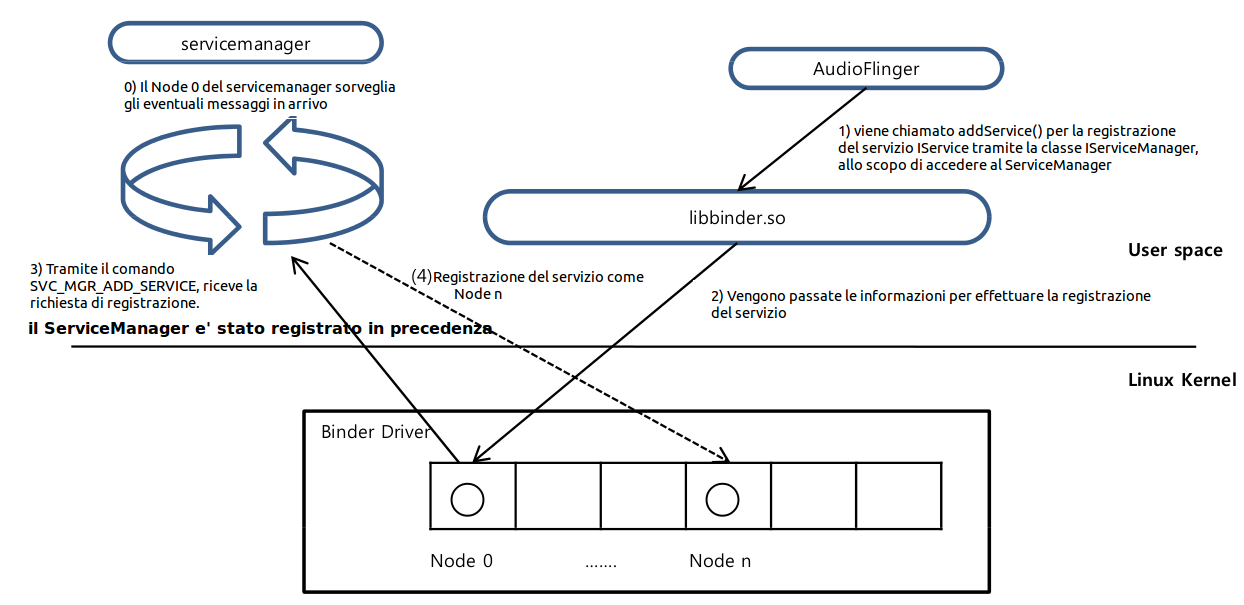
\includegraphics[scale=0.4]{img/korea/registration.png}}\\
\subfloat[][\textit{Visione High-Level del meccanismo di IPC. }]{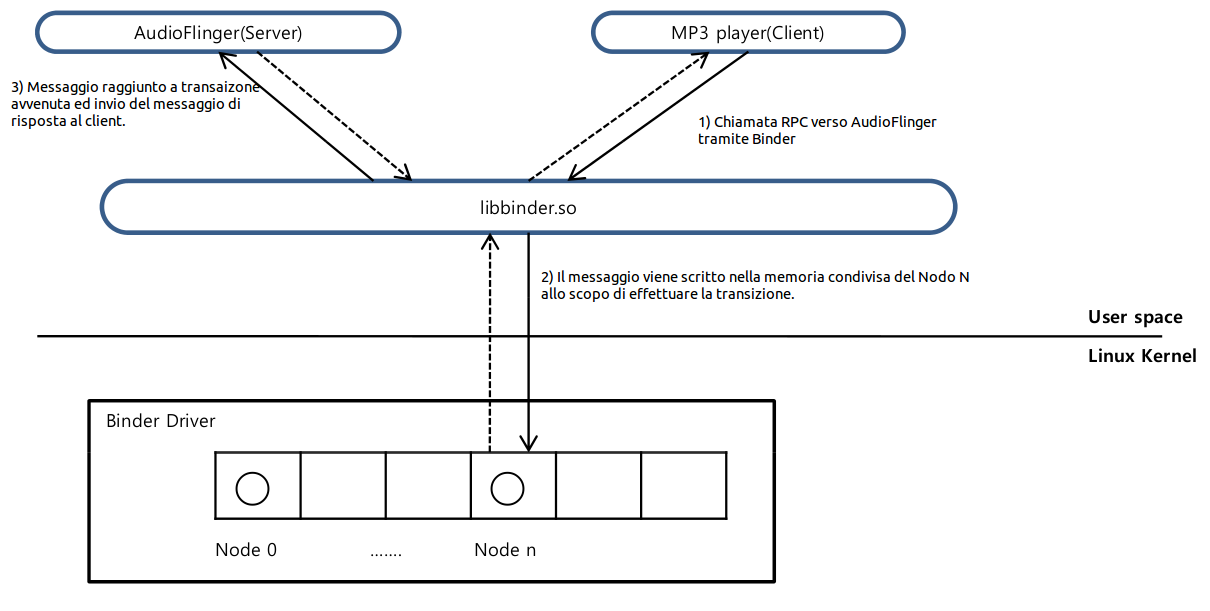
\includegraphics[scale=0.43]{img/korea/transact.png}}\\
\caption{\textit{Overview} generale dei meccanismi di comunicazione predisposti dal
Binder.
\url{http://www.aesop.or.kr/Board_Documents_Android_Frameworks/34984}}
\label{fig:androidbinderoverview}
\end{figure}
\end{list}

Mi focalizzerò ora su come avvenga la registrazione di un \textit{service} lato Java,
prendendo ad esempio quella del \texttt{\small PermissionController} definito
all'interno dell'\texttt{\small ActivityManagerService}, il quale tra l'altro si 
occupa anche della gestione degli eventi attinenti alle \textit{Activity} delle
API Java. All'atto dell'inizializzazione del servizio \texttt{\small ActivityManagerService},
oltre alle restituzione del \textit{context} di sistema tramite l'inizializzazione
\texttt{\small init},  avviene la chiamata alla funzione \texttt{\small setSystemProcess}
che inizializza il servizio \texttt{\small permission}.

Osservando la  Figura \vref{fig:androidbinderoverview}, possiamo ottenere una
visione generale di come ciò possa avvenire: sia il client sia il \textit{service}
condividono un'area di memoria grazie alla predisposizione dei
nodi tramite i quali effettuare la comunicazione.


\begin{figure}[p]
\centering
\subfloat[][\textit{Gerarchia delle classi lato Java/Service. }]{\includegraphics[scale=0.43]{img/modelio/Server.png}}\\
\subfloat[][\textit{Gerarchia delle classi lato codice chiamante. }]{\label{subfig:clientggl}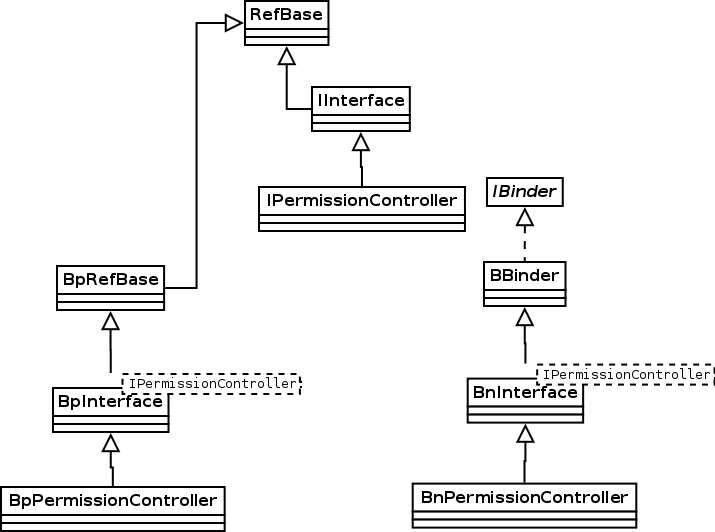
\includegraphics[scale=0.43]{img/modelio/Client.png}}\\
\caption{Visione \textit{High-Level} della gerarchia delle classi del sistema di IPC.}
\label{fig:highlevelhierarchy}
\end{figure}

In quanto:
\begin{center}
\texttt{\small Binder$_\mathtt{J}$ <: IPermissionController.Stub$_\mathtt{J}$ <: PermissionController$_\mathtt{J}$}
\end{center}
il costruttore di \texttt{\small PermissionController} provocherà l'invocazione
dei supercostruttori, tra i quali compare quello della classe madre \texttt{\small Binder}.
Quest'ultimo provoca l'invocazione del metodo nativo \texttt{\small init()}
che corrisponde alla chiamata della funzione \texttt{\small android\_os\_Binder\_init},
dove avviene l'associazione tra la classe Java e l'oggetto nativo \texttt{\small JavaBBinderHolder}.

Quest'oggetto a sua volta conterrà, tramite la variabile \texttt{\small mBinder},
un riferimento all'oggetto \texttt{\small JavaBBinder$_\mathtt{C}$} che, estensione
di \texttt{\small BBinder$_\mathtt{C}$}, conterrà un riferimento \texttt{\small mObject}
all'oggetto Java chiamante.

Faccio ora riferimento al codice di \texttt{\small ServiceManager} fornito nel Listato
\vref{lst:servicemanagerjava};
passando quindi alla procedura di ottenimento del \textit{Service Manager} lato Java,
ed in particolare all'invocazione del metodo nativo \texttt{\small getContextObject()}
implementato nel metodo \texttt{\small android\_os\_BinderInternal\_getContextObject},
subito dopo aver ottenuto il riferimento dell'oggetto \texttt{\small BpServiceManager}, lo
si processa all'interno del metodo \texttt{\small javaObjectforIBinder} dove, dopo
aver saltato i primi due controlli ed aver verificato il terzo, si creerà un
nuovo oggetto Java \texttt{\small BinderProxy$_\mathtt{J}$} che memorizzerà al
suo interno l'oggetto nativo ottenuto, e tramite il quale effettuare la richiesta
al Binder.



\begin{algorithm}[p]
\lstinputlisting[caption=$ $ServiceManager.java,label=lst:servicemanagerjava,language=Java]{srcs/ServiceManager.java}
\end{algorithm}

Riassumendo i passi successivi, non necessari per l'immediato completamento
della tesi\footnote{Le informazioni complete sono tuttavia fornite all'interno
del sito in Cinese \url{http://blog.csdn.net/tjy1985/article/details/7408698}.}, l'oggetto
ottnenuto lato Java tramite lo strato JNI verrà poi utilizzato come argomento
per il costruttore della classe \texttt{\small ServiceManagerProxy$_\mathtt{J}$}; 
quest'ultimo oggetto instaurerà poi lato Java l'effettiva comunicazione con il 
driver, grazie all'associazione di questo all'attributo \texttt{\small mRemote}.

Volendo ora mostrare come sia possibile registrare il servizio \texttt{\small PermissionController},
l'invocazione di \texttt{\small addService} provocherà la chiamata di un metodo
definito all'interno di \texttt{\small ServiceManagerNative.java}, il quale
causerà la transazione sull'oggetto \texttt{\small mRemote}, provocando una
procedura  di inserimento dell'oggetto \texttt{\small BBInder$_\mathtt{C}$}, 
non dissimile a quella già descritta per i \textit{service} nativi.
In fine si può osservare da codice come l'oggetto effettivamente fornito
al Binder sia quello precedentemente memorizzato in \texttt{\small mObject}.

In questo modo ho mostrato come sia possibile, da codice Java, generare oggetti
nativi che in seguito possano far riferimento all'oggetto generate.

\begin{algorithm}[p]
\begin{cpp}[ caption=$ $ Alcune funzioni JNI in \texttt{\small android\_util\_Binder.cpp},label=lst:androidutilbind]
static void android_os_Binder_init(JNIEnv* env, jobject obj)
{
    JavaBBinderHolder* jbh = new JavaBBinderHolder();
    if (jbh == NULL) {
        jniThrowException(env, "java/lang/OutOfMemoryError", NULL);
        return;
    }
    ALOGV("Java Binder %p: acquiring first ref on holder %p", obj, jbh);
    jbh->incStrong((void*)android_os_Binder_init);
    env->SetIntField(obj, gBinderOffsets.mObject, (int)jbh);
}

jobject javaObjectForIBinder(JNIEnv* env, const sp<IBinder>& val)
{
    if (val == NULL) return NULL;

    if (val->checkSubclass(&gBinderOffsets)) { ... }
    jobject object = (jobject)val->findObject(&gBinderProxyOffsets);
    if (object != NULL) { ... }
    object = env->NewObject(gBinderProxyOffsets.mClass, gBinderProxyOffsets.mConstructor);
    if (object != NULL) {
        LOGDEATH("objectForBinder %p: created new proxy %p !\n", val.get(), object);
        // The proxy holds a reference to the native object.
        env->SetIntField(object, gBinderProxyOffsets.mObject, (int)val.get());
        val->incStrong(object);
        //Omissis
    }
}

sp<IBinder> ibinderForJavaObject(JNIEnv* env, jobject obj)
{
    if (obj == NULL) return NULL;

    if (env->IsInstanceOf(obj, gBinderOffsets.mClass)) {
        JavaBBinderHolder* jbh = (JavaBBinderHolder*)
            env->GetIntField(obj, gBinderOffsets.mObject);
        return jbh != NULL ? jbh->get(env, obj) : NULL;
    }

    //Omissis
}

static jobject android_os_BinderInternal_getContextObject(JNIEnv* env, jobject clazz)
{
    sp<IBinder> b = ProcessState::self()->getContextObject(NULL);
    return javaObjectForIBinder(env, b);
}
\end{cpp}
\end{algorithm}

\subsubsection{Invocazione di metodi Java da Native Code}\label{subsec:invoke}
\begin{figure}[thp]
\centering
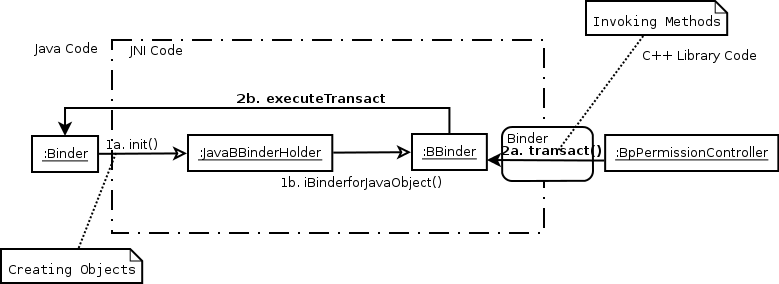
\includegraphics[scale=0.65]{img/modelio/cpplevel.png}
\caption{\textit{Visione dell'interazione tra oggetti interagenti nel corso dell'IPC per i}
service \textit{Java}.}
\label{fig:binderlowlevel}
\end{figure}
Voglio mostrare come sia possibile effettuare l'invocazione del metodo \texttt{\small checkPermission}
lato Java da parte di codice nativo.

Sapendo che:
\begin{center}
\texttt{\small Binder$_\mathtt{J}$ <: IPermissionController.Stub$_\mathtt{J}$ <: PermissionController$_\mathtt{J}$}
\end{center}
abbiamo che tale metodo dichiarato all'interno della classe \texttt{\small PermissionController}
mostrata in precedenza nel Listato \vref{lst:stubipermissioncontroller}, verrà
richiamato dal metodo \texttt{\small onTransact} definito in \texttt{\small Stub},
a sua volta richiamato dal metodo \texttt{\small executeTransact} definito all'interno
della classe \texttt{\small Binder}.

Ricercando ora come tale metodo possa essere richiamato a livello di JNI,
si scopre che questa invocazione viene consentita all'interno del metodo
\texttt{\small onTransact} come definito nella classe \texttt{\small JavaBBinder},
a sua volta richiamato dal metodo \texttt{\small transact} definito all'interno
della classe \texttt{\small BBinder}, dove:
\begin{center}
\texttt{\small BBinder$_\mathtt{C}$ <: JavaBBinder$_\mathtt{C}$}
\end{center}

Questo metodo verrà poi richiamato da del \textit{main loop} fornito lato JNI dal 
\texttt{\small system\_server}, come già mostrato in precedenza per i \textit{service}
nativi.


